\graphicspath{{chapter_background/}}
\chapter{Background}
\label{chapter:background}

This chapter gives an introduction to the volumetric representation we
use for encoding 3D geometry, along with some of the algorithms
associated with volumetric data, such as voxelisation and surface
extraction. This thesis assumes a basic knowledge of deep learning,
such as the typical layers that might be used to construct a
Convolutional Neural Network (CNN).

\section{3D Volumes and Volumetric Algorithms}
\label{sec:background:volumes}

Typically, 3D models are provided as a mesh, defined by vertices and
faces, in a particular file format such as \textit{Wavefront
  Obj}. These files typically contain additional data, such as texture
mapping coordinates and surface normals. However, to represent the
shape of an object, only the mesh is required. Directly regressing the
vertices for this mesh using a CNN, along with a predefined set of
faces, would be a very elegant approach to 3D face
reconstruction. However, such an approach has never been demonstrated
before, and it is likely that it isn't possible using a CNN unless the
dimensionality of the problem is first reduced (hence 3DMM).

An alternative approach to representing the shape of an object is to
encode it in a three dimensional volume. Typically, each voxel stores
an intensity value, much like a grey scale image, collected using an
MRI scanner for example. However, by storing only binary values, we
can encode the 3D shape of an object. This may be thought of as a 3D
matrix, where \textit{inside} the object is denoted by a one, and
\textit{outside} is denoted with a zero. This allows us to constrain
the problem of 3D face reconstruction to one that spatial, avoiding
the need to transfer knowledge to a parametric or Euclidean space.

\begin{figure}
  \begin{tabular}{ccccc}
    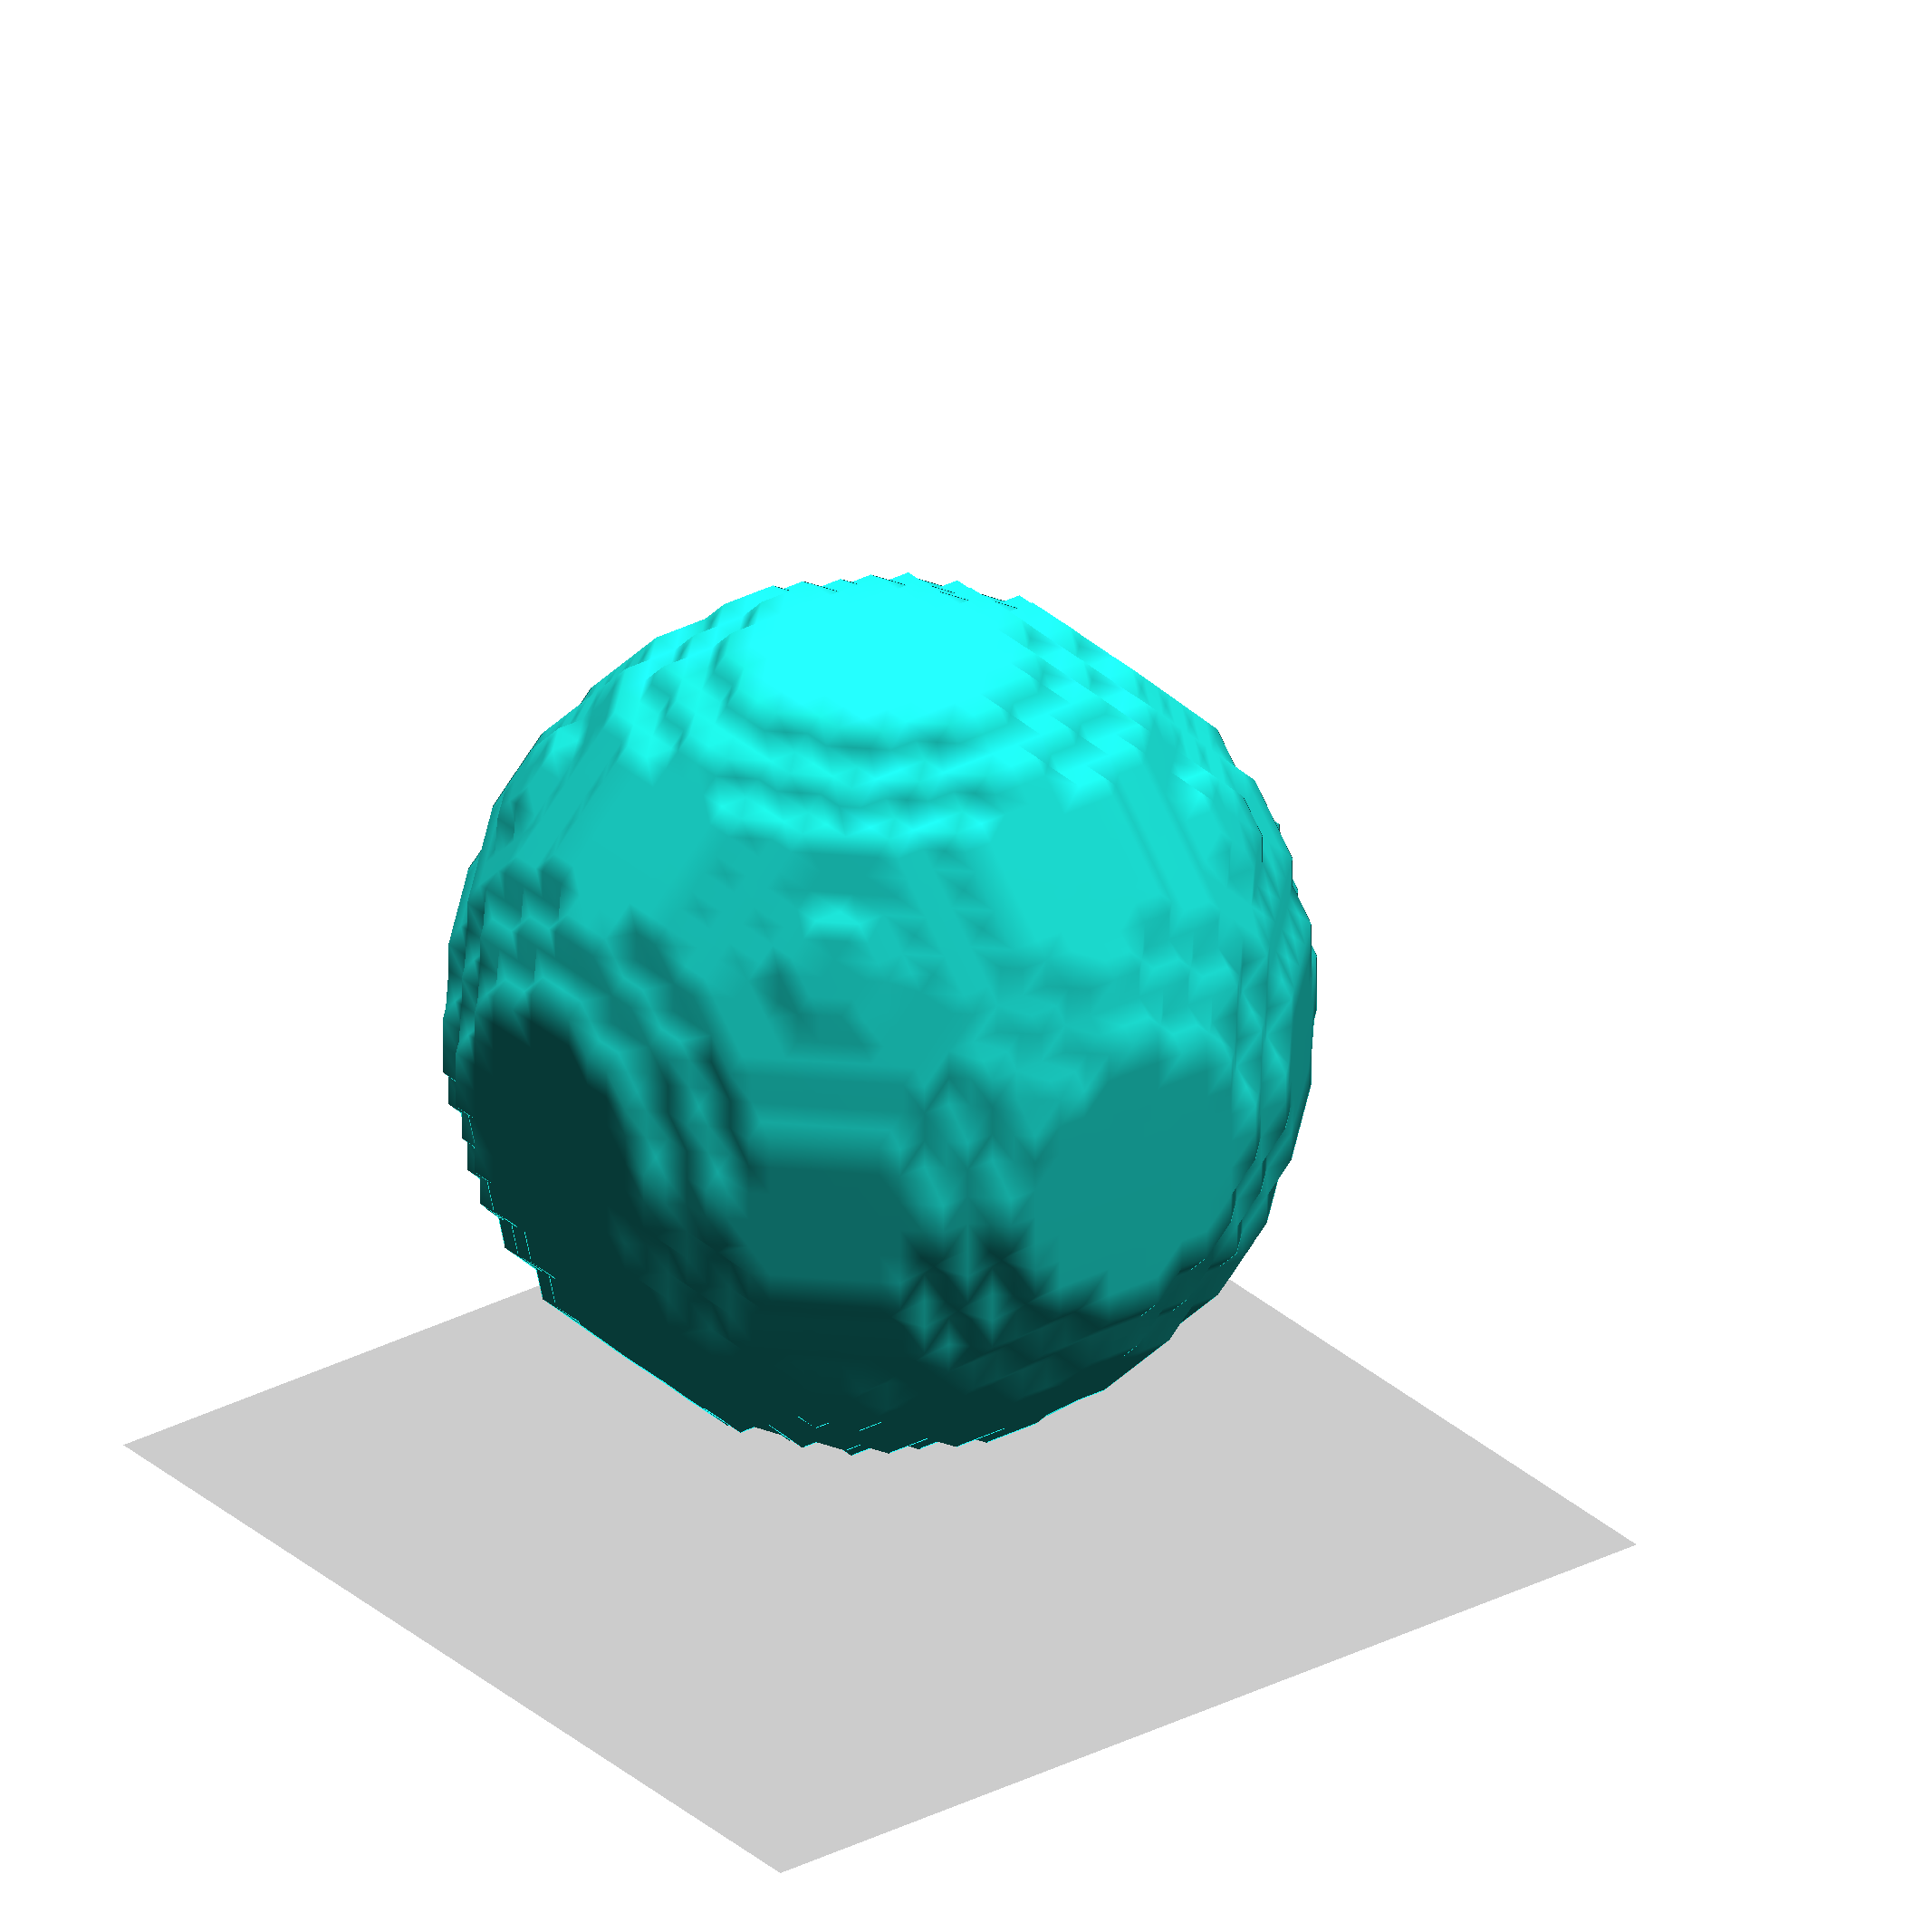
\includegraphics[width=0.18\linewidth]{chapter_background/img/binary_32x32x32.png} &
    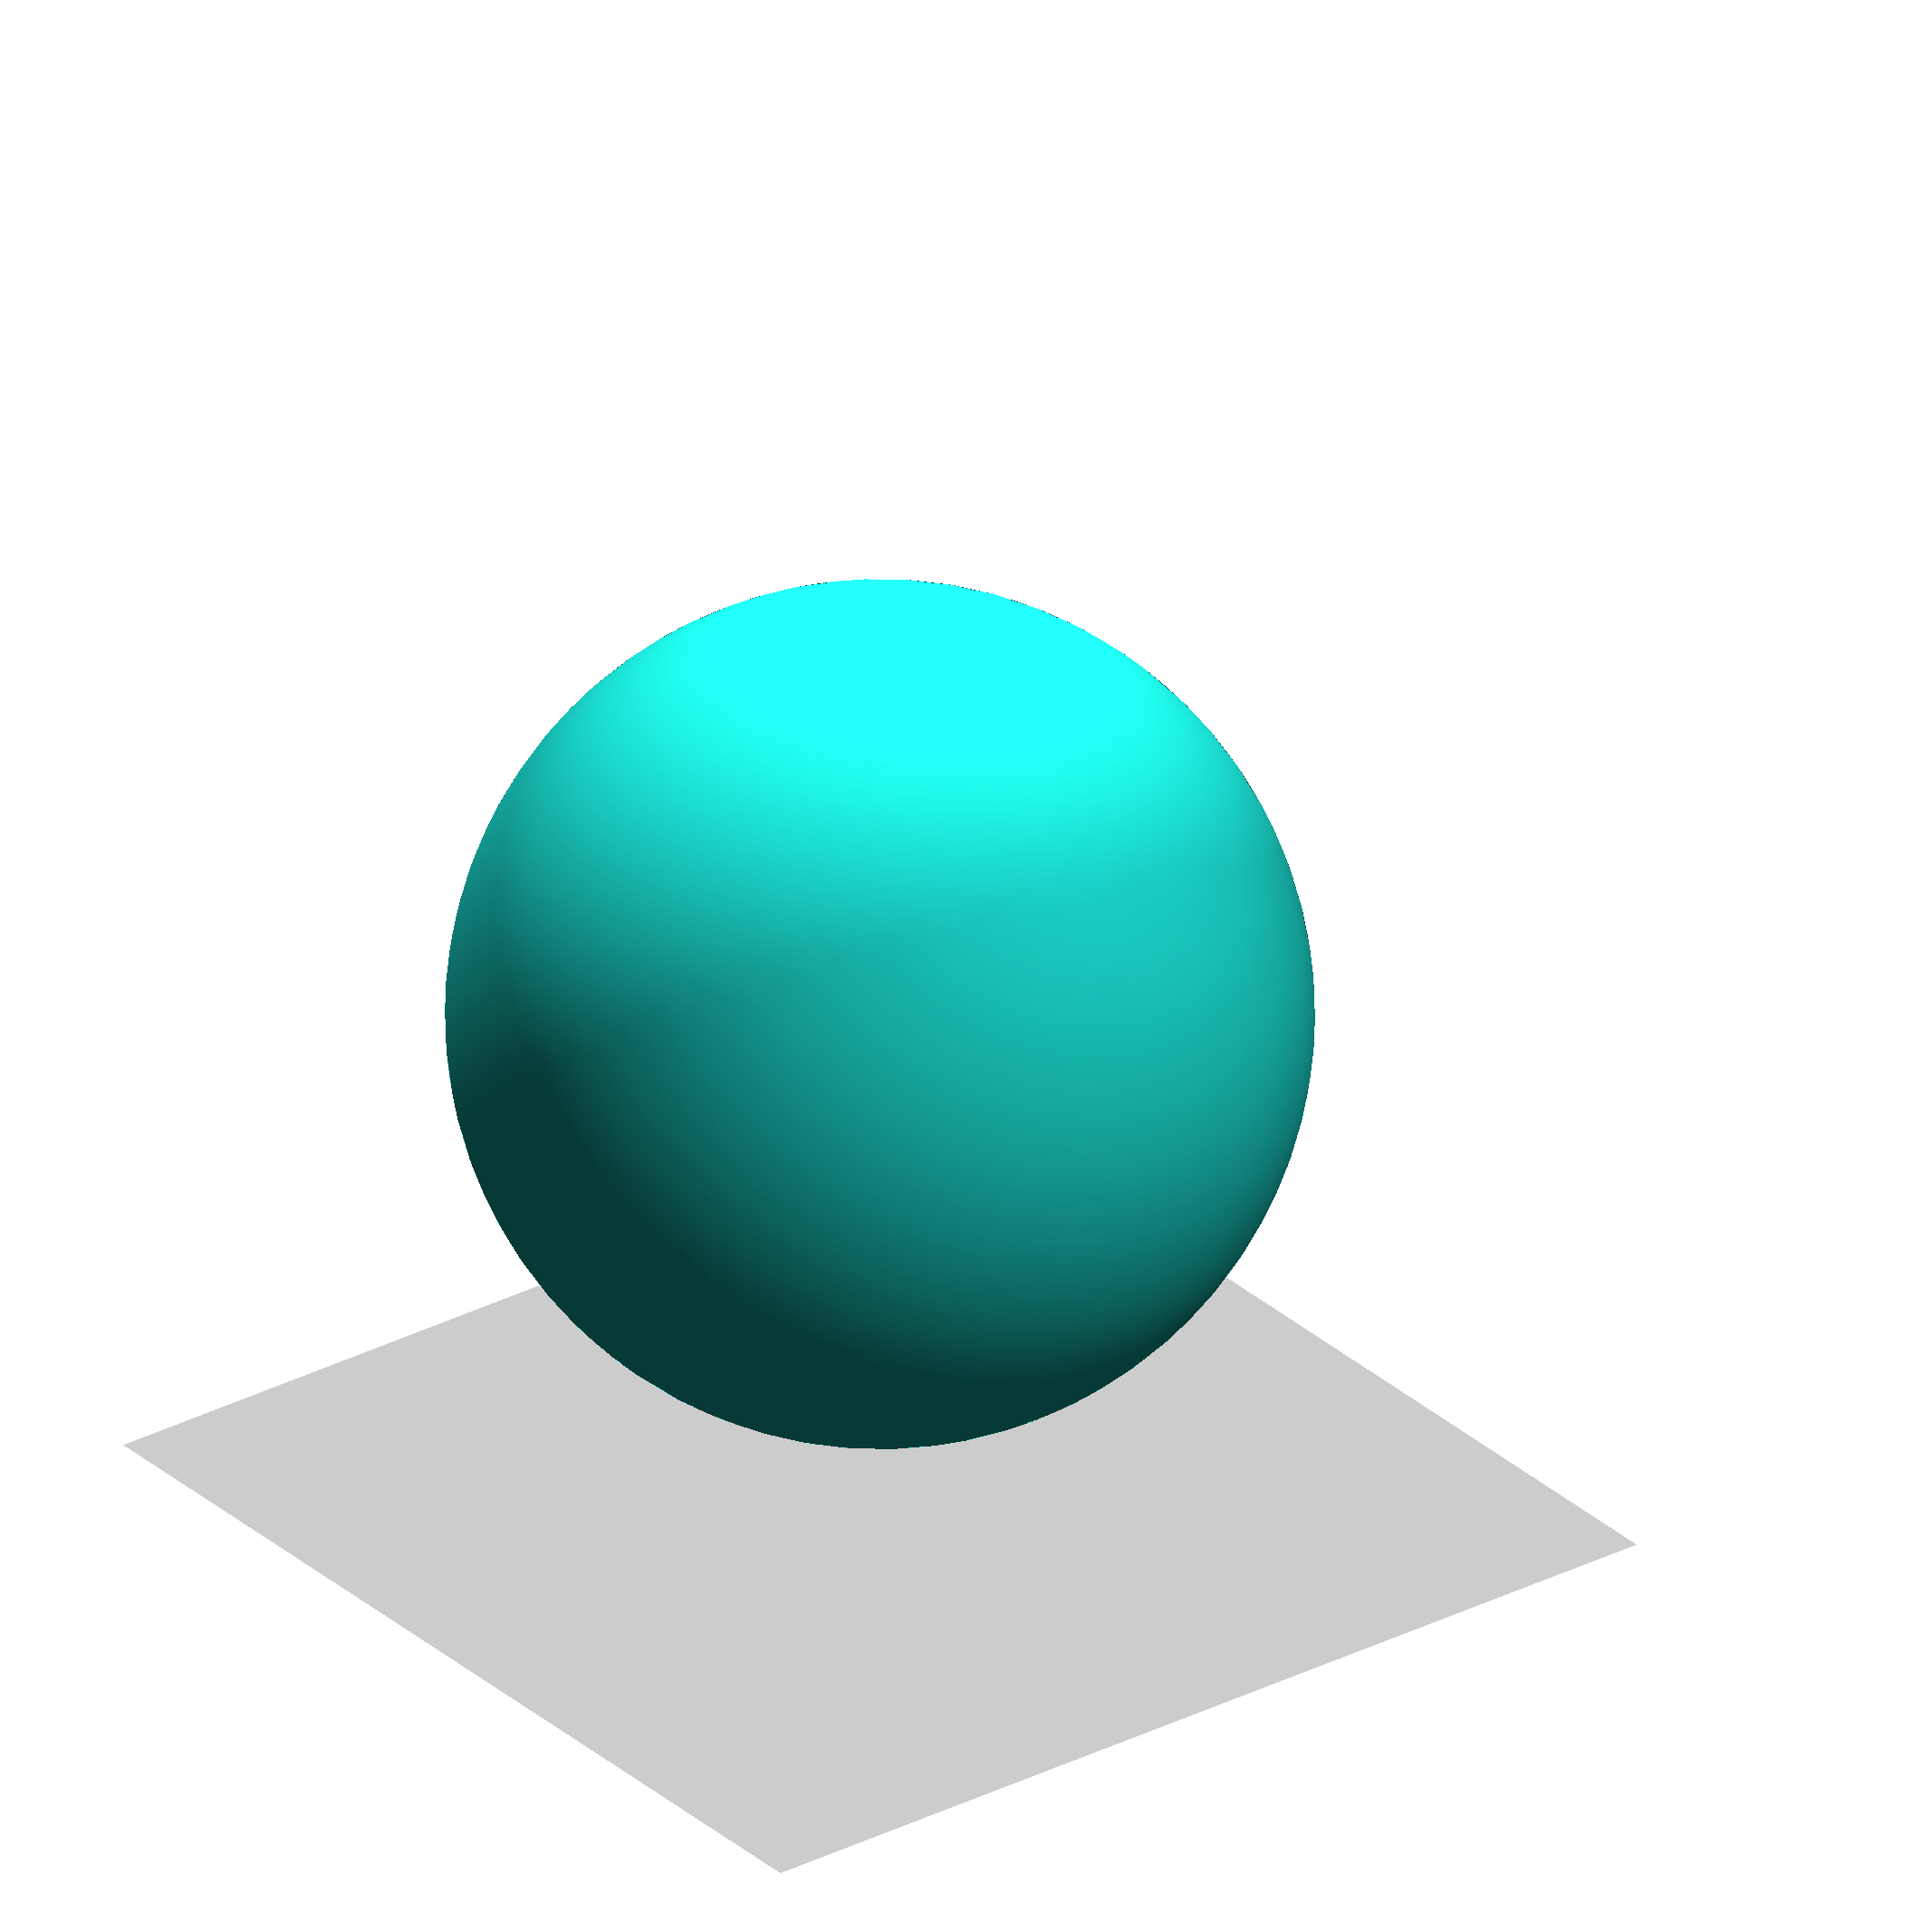
\includegraphics[width=0.18\linewidth]{chapter_background/img/real_32x32x32.png} &
    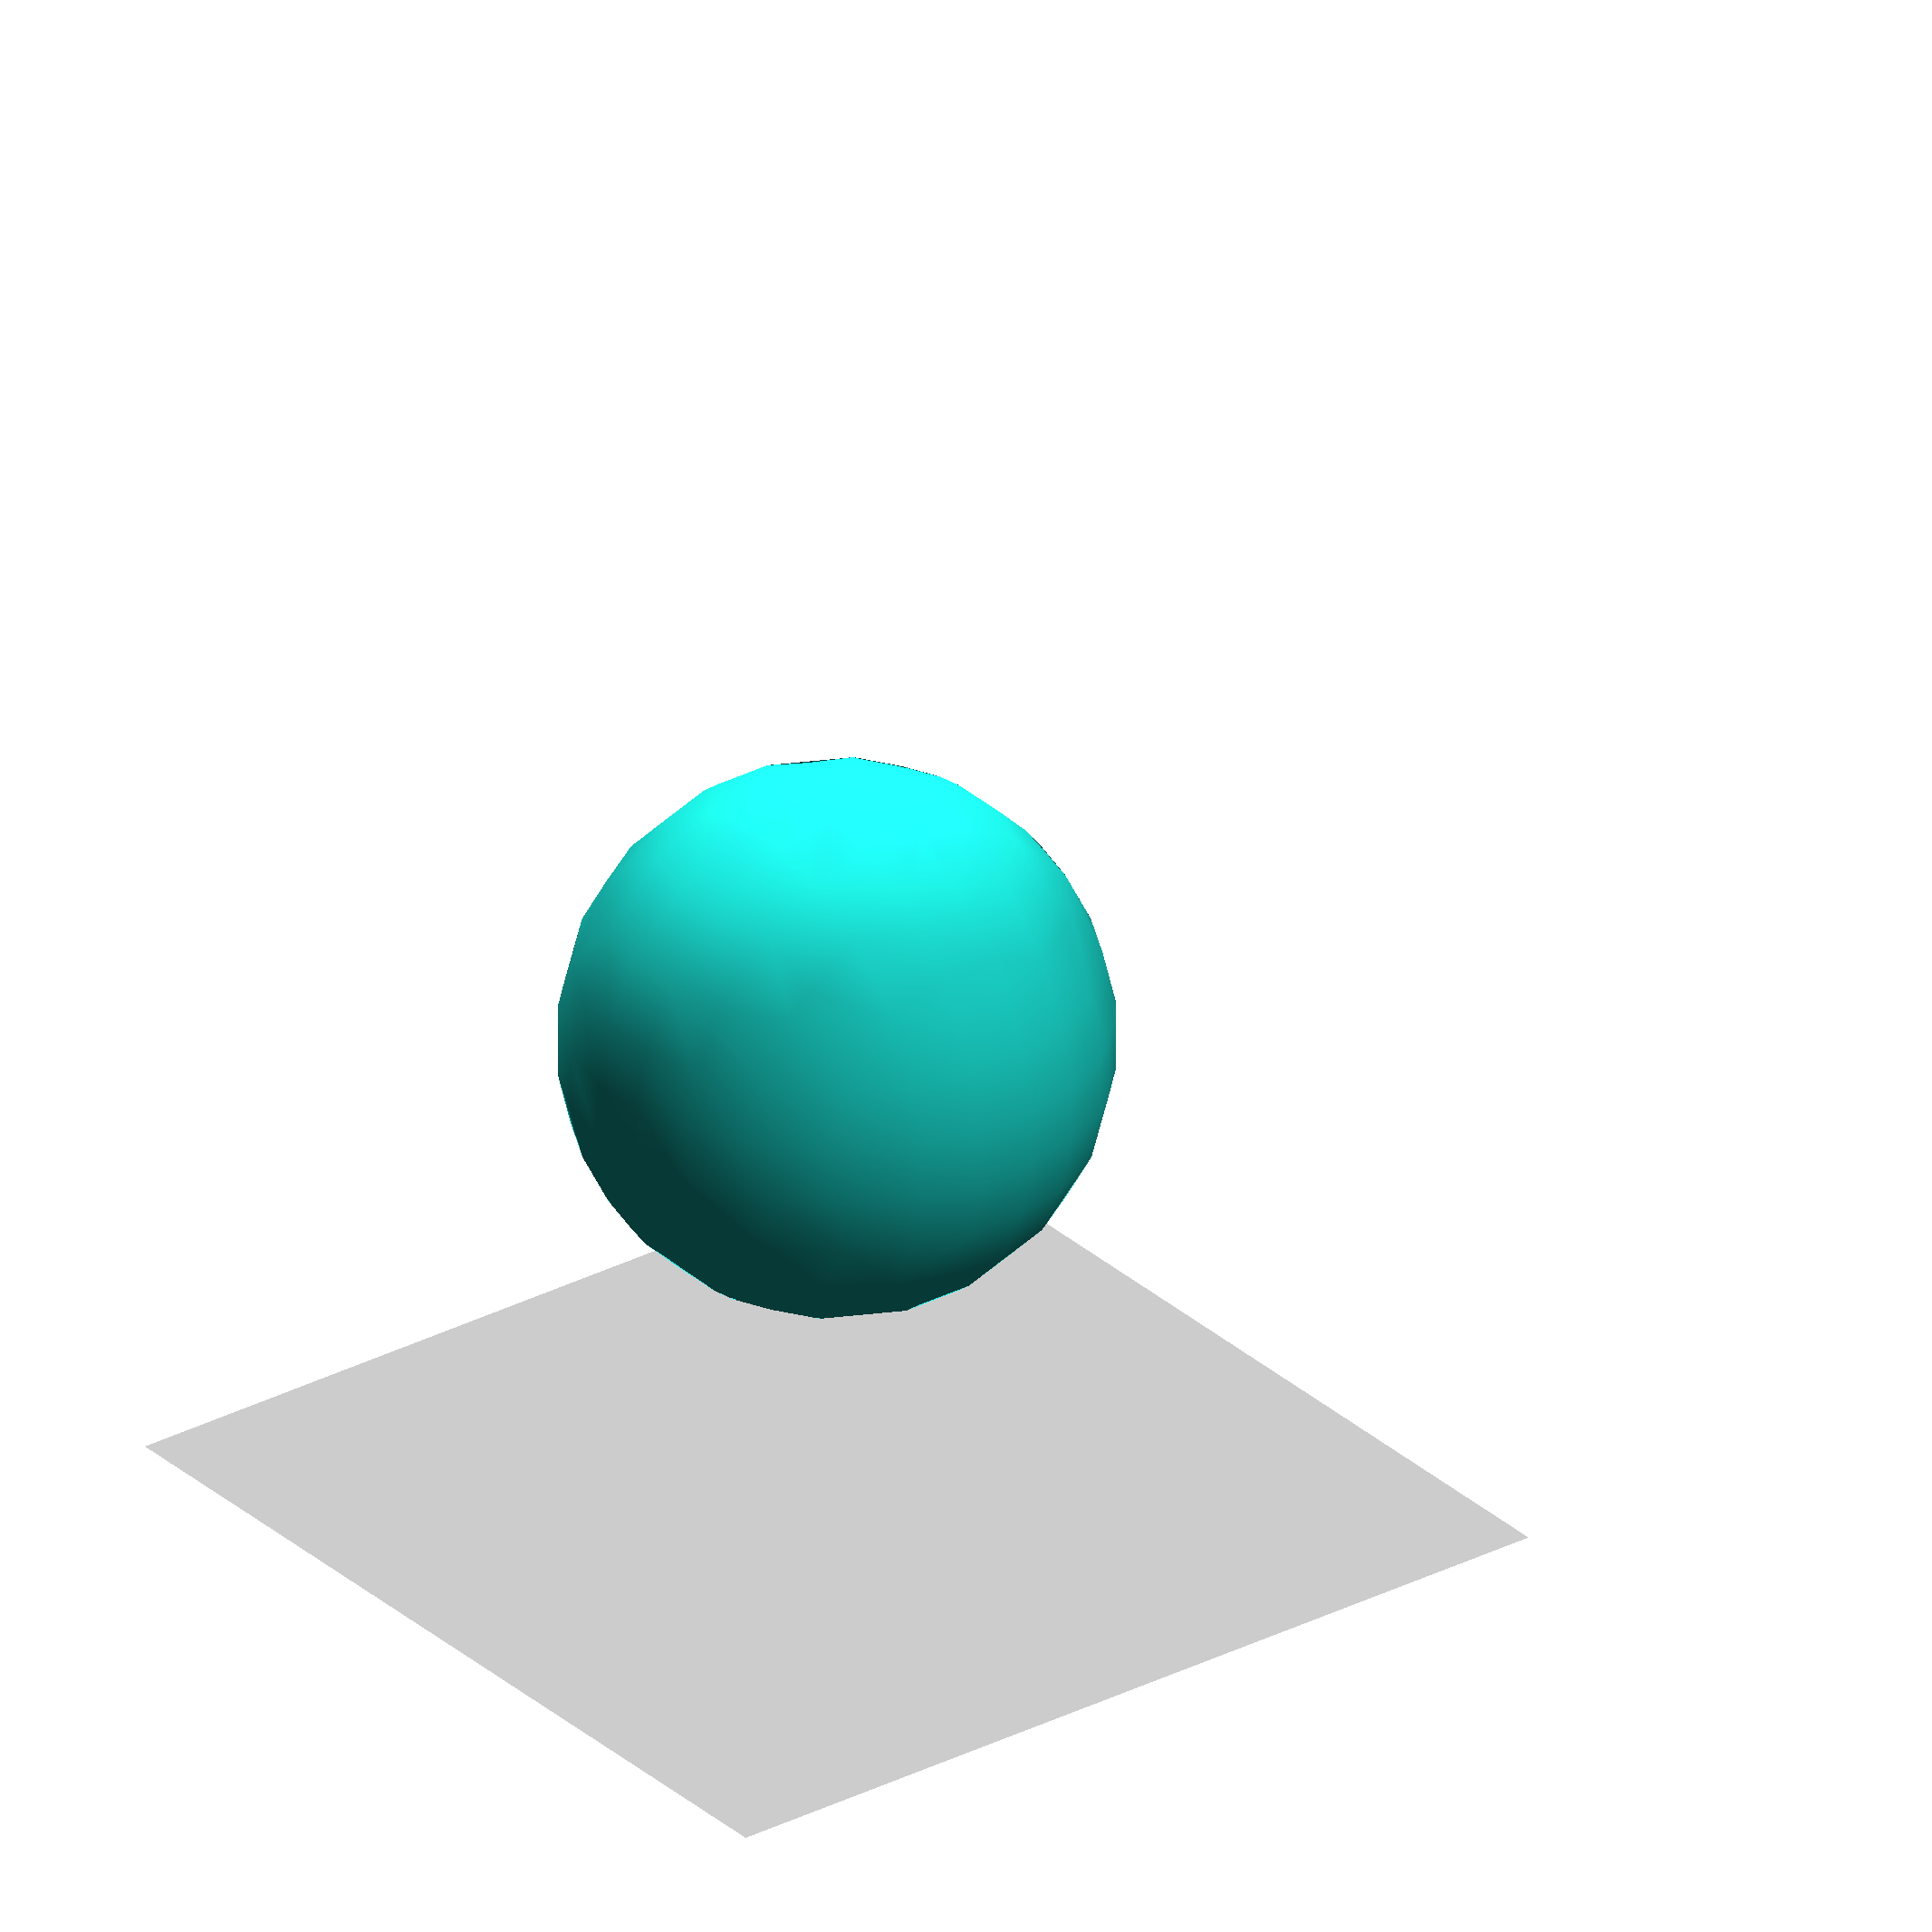
\includegraphics[width=0.18\linewidth]{chapter_background/img/real_16x16x16.png} &
    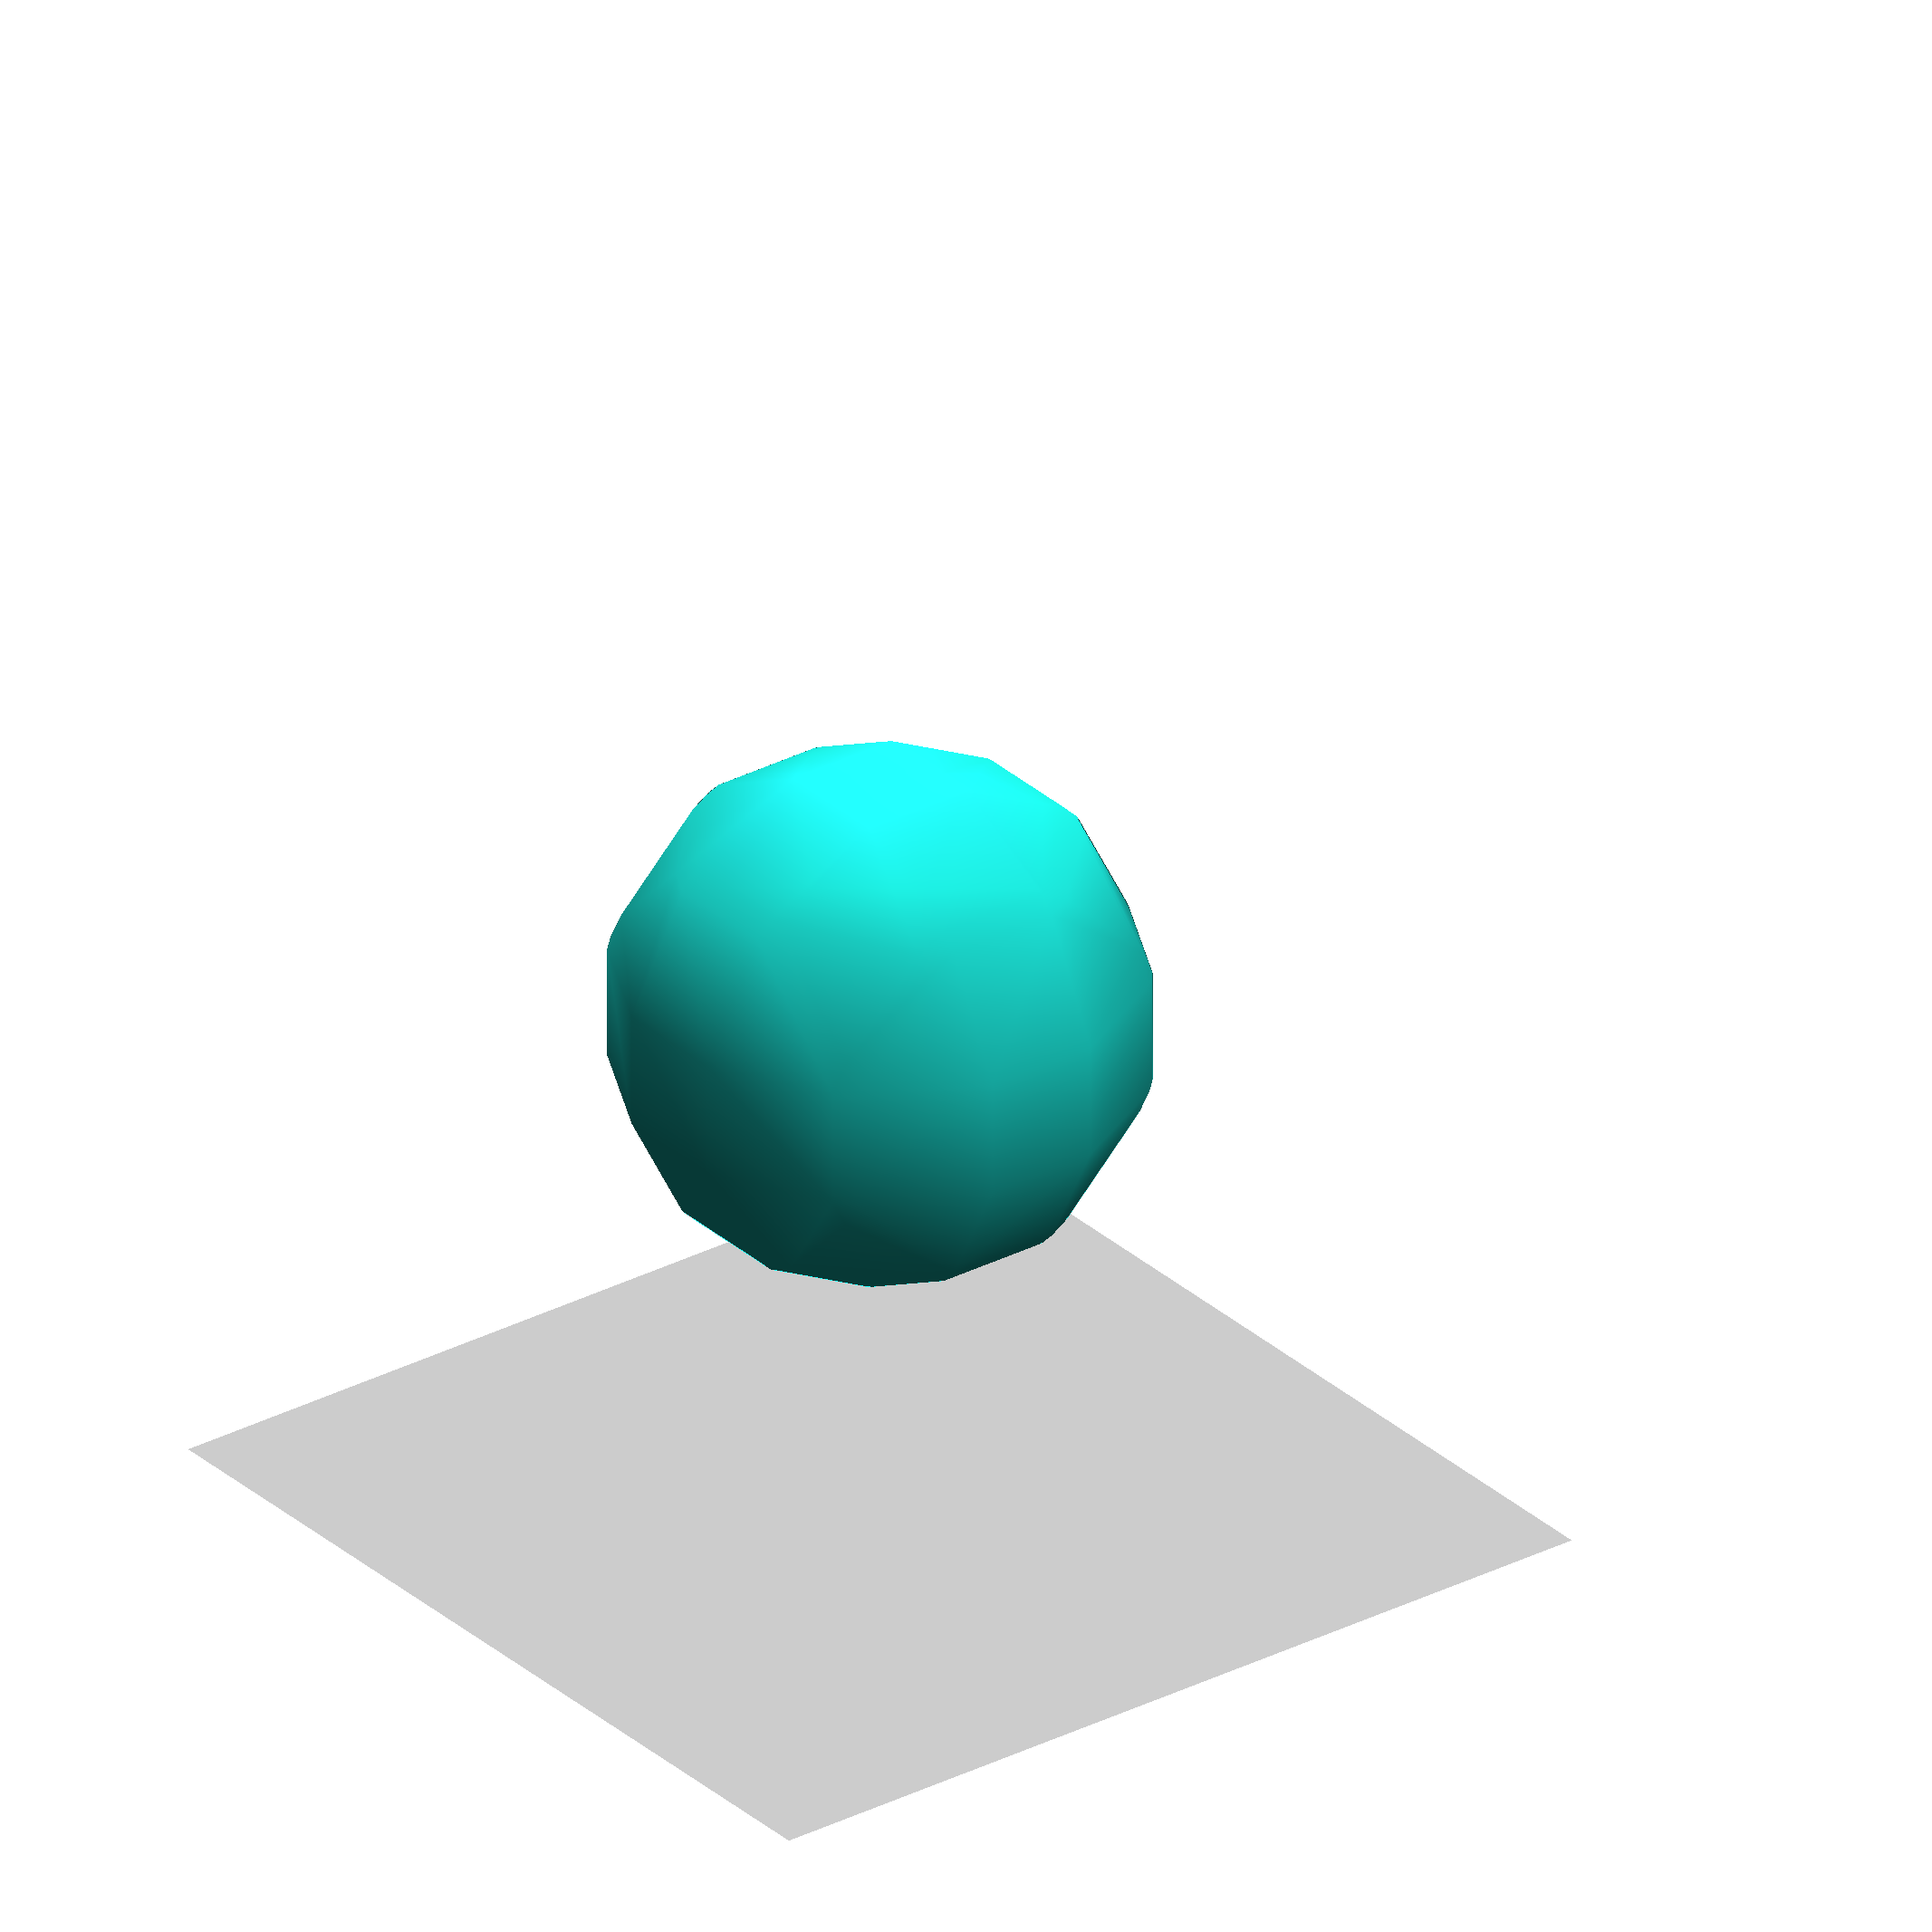
\includegraphics[width=0.18\linewidth]{chapter_background/img/real_8x8x8.png} &
    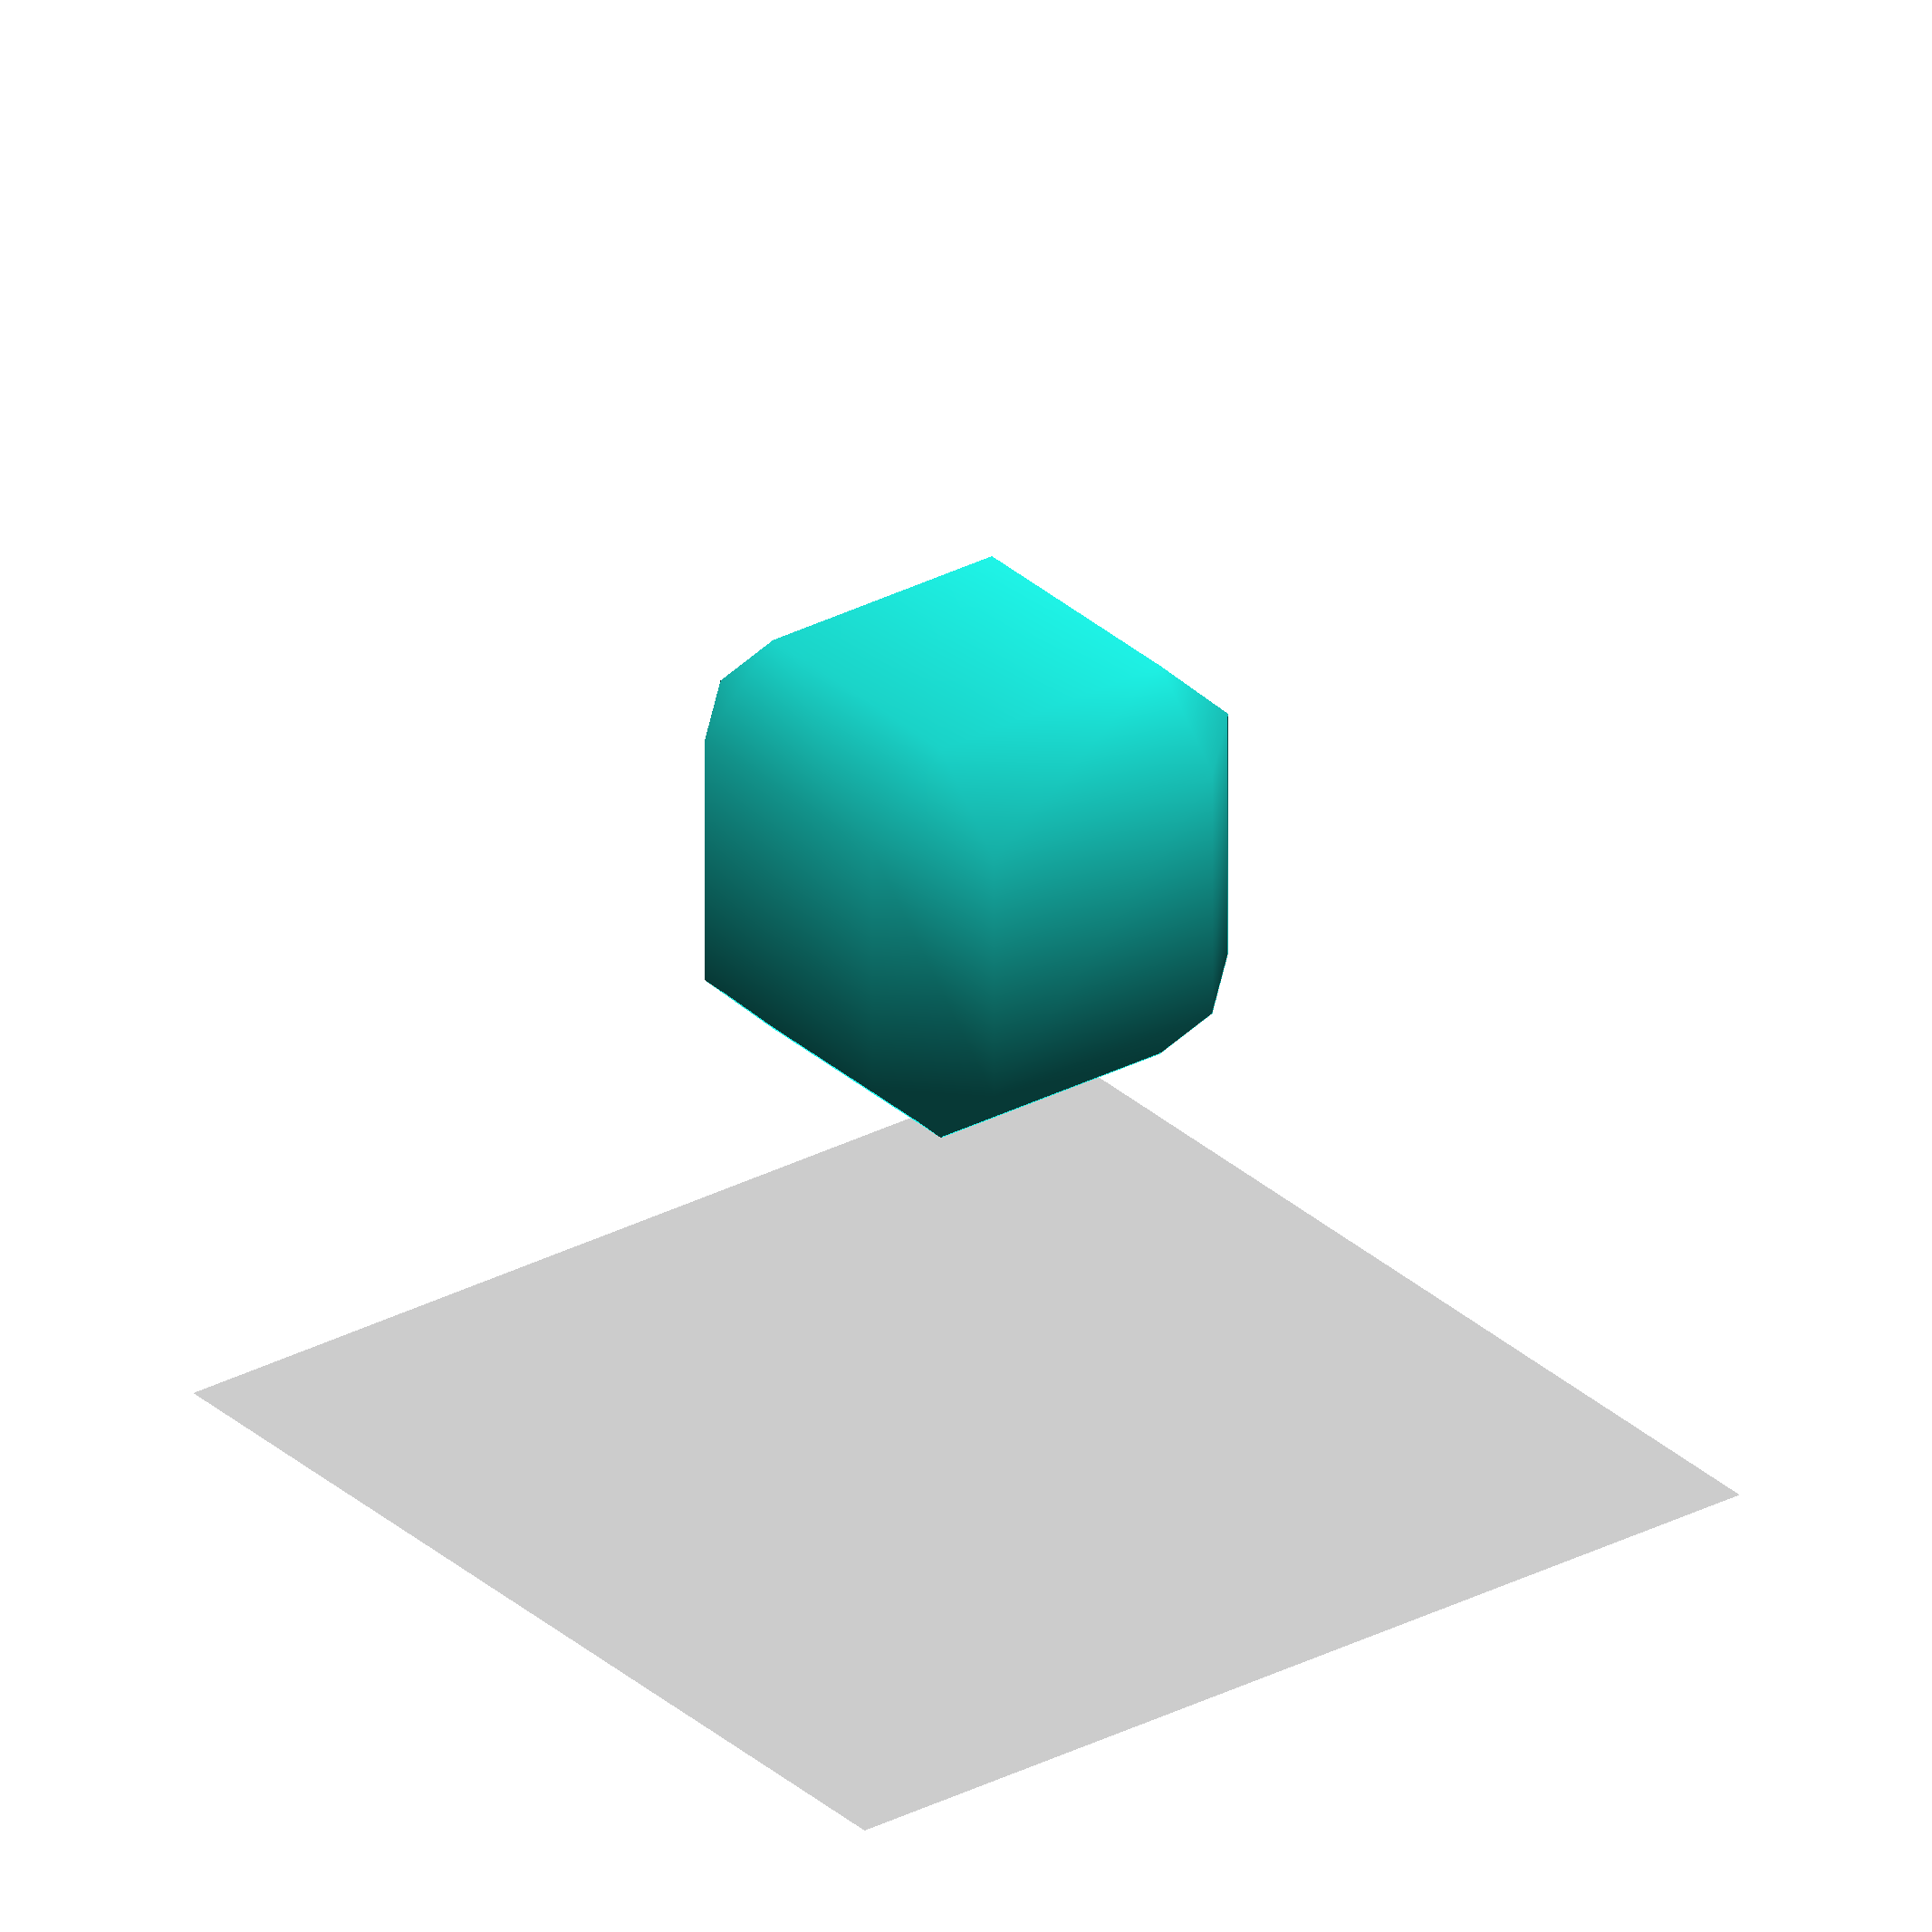
\includegraphics[width=0.18\linewidth]{chapter_background/img/real_4x4x4.png}
    \\
    Binary & Real & Real & Real & Real \\
    $32^3$ & $32^3$ & $16^3$ & $8^3$ & $4^3$ \\
  \end{tabular}
  \caption[Volumetric antialiasing at different resolutions]{A
    volumetric sphere, with and without antialiasing, at several
    different resolutions.}
  \label{fig:background:volquality}
\end{figure}

\subsection{Voxelisation}

The process of transforming a mesh into a volumetric structure is
referred to as voxelisation. Intuitively, this voxelisation process
discretises the mesh. It is no longer possible to reproduce a
non-integer form of the original mesh - a surface noticeably
constructed out of small cubes. Ideally, there should be minimal
visual degradation between viewing the original mesh and the voxelised
object, otherwise, how would it be possible to encode detail?  Just as
anti-aliasing is possible in 2D graphics, it is also possible with 3D
volumes. This is achieved by using real numbers inside a voxel,
instead of just a binary value.  This results in very low distortion,
provided the resolution is sensibly selected. This is shown in
Figure~\ref{fig:background:volquality}, where a sphere encoded using
binary values is clearly built out of cubes, where as even a small
real value volume remains representative.

Generating a 2D image from 2D vector graphics (such as polygons) is
called rasterisation. This involves tracing a ray while counting the
number of line intersections. If the count is odd, colour in pixel and
move onto the next. If the count is even, just move onto the next
pixel. Voxelisation follows a similar idea, except it is performed in
three dimensions instead of two. This is done by tracing rays through
the X, Y and Z planes separately to produce three separate
volumes. These volumes are then combined in some way, typically by
ensuring each XYZ coordinate has been set in at least two volumes
(voting). We show this visually in
Figure~\ref{fig:background:voltracing}, where error (shown in red) has
been introduced by only voxelising the Stanford
Bunny\footnote{http://graphics.stanford.edu/data/3Dscanrep} from a
single direction.

\begin{figure}
  \centering
  \begin{tabular}{ccccc}
    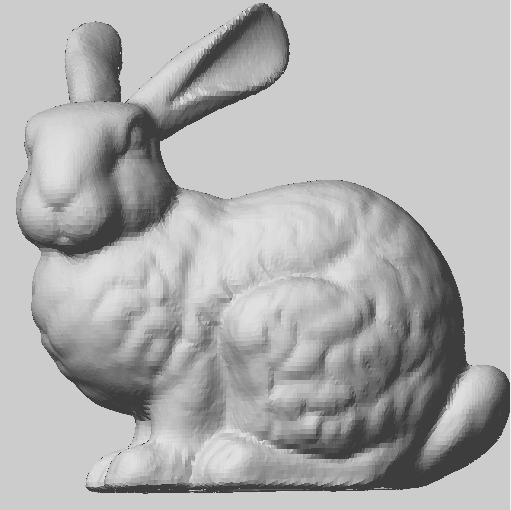
\includegraphics[width=0.17\linewidth]{imggen/vox_xyz/bunny_original.png} &
    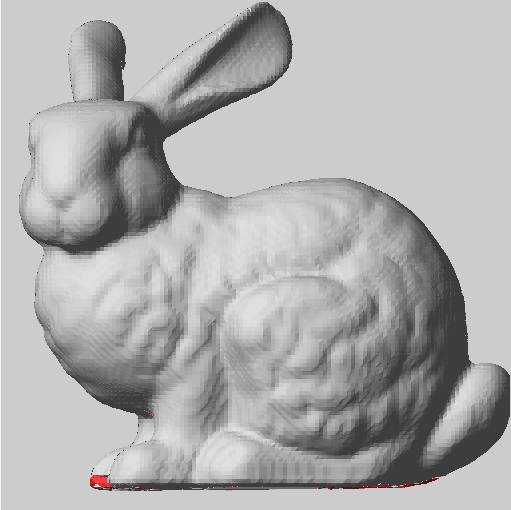
\includegraphics[width=0.17\linewidth]{imggen/vox_xyz/bunny_voxX.png} &
    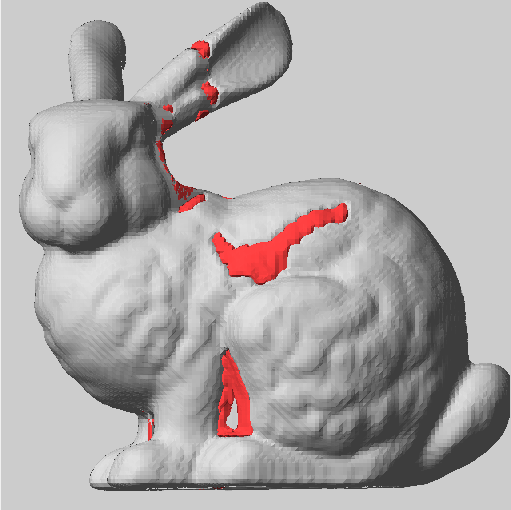
\includegraphics[width=0.17\linewidth]{imggen/vox_xyz/bunny_voxY.png} &
    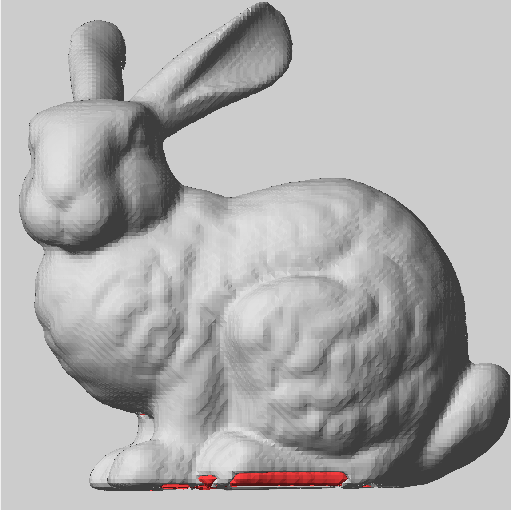
\includegraphics[width=0.17\linewidth]{imggen/vox_xyz/bunny_voxZ.png} &
    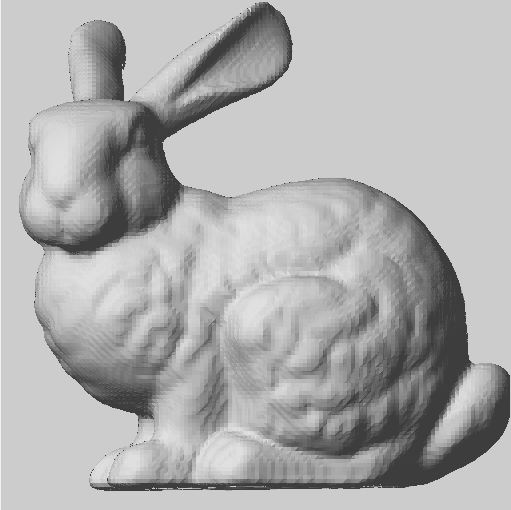
\includegraphics[width=0.17\linewidth]{imggen/vox_xyz/bunny_voxXYZ.png} \\
    Original & Voxelised & Voxelised & Voxelised & Voxelised \\
    Mesh     & Traced X  & Traced Y  & Traced Z  & Traced XYZ \\
  \end{tabular}
  \caption[Voxelisation error due to limiting ray tracing
  directions]{Voxelised results of the Stanford Bunny (original shown
    on left). The first three volumes have been voxelised by tracing
    from either X, Y or Z directions. The final volume (right most) is
    generated by voting. Red patches fill in voxels which have been
    missed. Each volume is $128^3$ in size.}
  \label{fig:background:voltracing}
\end{figure}

\subsection{Surface Extraction}

Surface extraction is the process of extracting a mesh which encloses
a 3D object represented in volumetric space. Occasionally such methods
require thresholds to extract separate regions of the volume, for
example, in an MRI scan, where the brain  needs to be visualised
independently of the skull (and hence, independently extracted from
the volume).

Perhaps the most popular method for computing the isosurface of a
volume is Marching Cubes~\cite{lorensen1987marching}, developed in
1987. The algorithm traverses through all voxels, using the value of
eight neighbouring voxels to form eight binary values, a single
byte. This byte can be used to lookup a known polygon configuration
from a table of $2^8 = 256$ entries. However, in the first version of
Marching Cubes, only 15 unique polygon configurations were
stored. This lead to cases of ambiguity when performing a lookup for
certain voxel configurations. The side effect of this is that meshes
would sometimes end up having holes in
them. In~\cite{chernyaev1995marching}, additional unique
configurations were proposed, leading to a total of 33. This removes
the ambiguity, and results in the meshes being closed or \textit{water
  tight}.


\subsection{Size, Compression and Formats}
\label{sec:background:volstorage}

There are many more factors which have to be considered when working
with volumetric representations of objects, as opposed to a standard
mesh.

To start with, the \textbf{size} of the volume (in terms of bytes)
grows much more rapidly than it would in a 2D image. In order to
represent a sensible amount of depth in a $128 \times 128$ image, a
volume of $128^3$ voxels is likely needed. If this is uncompressed and
encoded as bytes, it will require 2MB of storage. Scale this up to a
dataset of maybe 50,000 samples, use a slightly larger volume, and it
is clear that this may begin to cause problems.

One solution might be to compress the volumes. However, compression
introduces a significant computational overhead. It is a common trade
off between processing power, available storage and I/O speeds. While
compression of images has come a long way (even JPEG decoding is
hardware accelerated on some platforms now), the same is not true for
3D volumes. Generic file compression options are of course available
(Run Length Encoding, Huffman Coding and LZ77, just to name a few),
but on large volumes being read many times per second, the CPU could
easily become the bottleneck. In this work, we do not compress the
volumes and instead use large SSDs to store our volumetric training
data.

The format in which the volume is stored is another important
consideration. There are many formats for storing volumetric
data. Typically, these formats have been developed for the medical
field for use with MRI, CT scans and the like. As such, these formats
often include space for details such as patient information, along
with a metadata describing the resolution and bit depth of the
volumetric data. An argument can be made that none of this information
is required if the volumetric representation is used as an
intermediary state and doesn't have to be processed by
\textit{humans}. This applies to the work presented in this
thesis. The volumetric representation used in the work described
throughout this thesis is a contiguous array of bytes, which can be
very efficiently read into memory.

\section{Deep Learning Frameworks}

While designing and developing a framework to work with deep neural
networks \textit{might} be an interesting thought experiment for some,
it is far from the focus of this thesis. This section serves a brief
acknowledgement and justification for the choice of deep learning
framework used. The work presented throughout this thesis was
developed primarily under the Torch~\footnote{\url{http://torch.ch/},
  except for the work on facial part segmentation, which was developed
  under Cafe~\cite{jia2014caffe}}. There are a number of reasons for
this, but to name just a few:

\begin{enumerate}
\item Efficient GPU support. This is important, of course, in any
  framework intended for deep learning. Torch enables networks to be
  run in parallel (for speed) or sequentially (for additional memory)
  across multiple GPUs.
\item Elegant memory backend. Data can be loaded directly into memory
  and views can be applied to create $N$-dimensional Tensors without
  shuffling memory. This is very important when reading in large
  volumetric training samples.
\item Multithreading. The trade offs between I/O and CPU are discussed
  in more detail in Section~\ref{sec:background:volstorage}. However,
  regardless of how the data is optimised (in terms of compression or
  just raw data), volumes are big. Loading them sequentially and
  applying augmentation, even on very fast hardware, remains a
  computationally expensive task.
\end{enumerate}

%%% Local Variables:
%%% TeX-master: "../thesis"
%%% End:
